\documentclass{optica-article}
\journal{opticajournal} % for journals or Optica Open
\articletype{Research Article}
\usepackage{lineno}
\usepackage{verbatim}
\usepackage{graphicx} %immagini ecc
\usepackage{float}
\usepackage{hyperref}

\begin{document}

\title{ \begin{huge}
\textbf{NaoChallenge23 Technical Relation} 
\end{huge} }

\author{\centering NaoNexus}

\noindent
\textbf{FOR MORE INFO:} \\

\noindent\textit{Visit our} \href{https://www.naonexus.altervista.org/naochallenge2023/index.html}{website}



\noindent \textit{View our} \href{https://github.com/NaoNexus/ChallengeNao23}{repository}

\noindent\textit{Write an email at: }\email{socialnaonexus@gmail.com}

\bigskip

\begin{figure}
    \centering
    
\includegraphics[scale=0.05]{figures/logo.png}
    \label{fig:logo_con_scritta}
\end{figure}

\tableofcontents

\vspace{10pt}

\newpage

\begin{abstract*} 
\vspace{7pt}
\noindent
\\In this year's \emph{NaoChallenge} it was decided to develop two main projects oriented to sustainability and green energy. The \emph{mission} is to bring sustainability to everyone making it more accessible and easier to understand. These projects introduce people to the world of solar energy and their aim is to prevent energy waste in big infrastructures.\\

\section{METHODOLOGY AND TECHNOLOGIES USED}\label{sec:methodology_technologies}
As a big group there was a necessity to keep track of the tasks and keep everyone in sync with the latest developed software, for this reasons two important technologies were used: \emph{GitHub} and \emph{Notion}.

\subsection{DevOps with Notion and Agile methodology}\label{sec:devops_notion}
To work on the project and keep track of the progress made the team used \emph{Notion}, a collaborative note-taking software. The term \emph{DevOps} comes from the last part of \emph{software development} and \emph{technology operations} and its aim is to improve the collaboration end-to-end. With the web application Notion, which offered many useful tools such as task management, project tracking and to-do lists, the team has always been organized and focused on the work to do each session. This collaboration platform also integrates wikis and databases, creating all-in-one workspaces for notetaking and data management. The projects were managed with \emph{Agile} methodology, the problems were split into smaller tasks that were then distributed to the team members, this brought to an increased efficiency in software development and faster developing times.

\subsection{GitHub}\label{sec:git_hub}
GitHub is a powerful service that helped us store and manage our code. It is a website and cloud-based Git repository hosting service that essentially helps the user keep track of the changes made to the code thanks to \emph{version control}.\\
Through \emph{branching} and \emph{merging} each member was able to safely work on the code avoiding the direct modification of the original version. All of the changes made can eventually be reverted if they break the algorithm.

\bigskip

\noindent
\textbf{PRESENTING TWO PROJECTS}

\bigskip
\noindent
The first project uses NAO as an \emph{assistant} in a building. NAO is connected to a phone through an \hyperref[sec:domotics_server]{HTTP server}. Users can connect the phone to the server and send environmental data collected through an external \hyperref[sec:domotics_sensor]{sensor}. When NAO receives the environmental data he then manages the building's \hyperref[sec:domotics_domotics_server]{domotics} by turning on or off the \emph{lights}, raising or lowering the \emph{blinds} or turning on or off the \emph{heating}.\\

%\bigskip
%\vspace{10pt}

\vspace{7pt}
\noindent
The second project required the collaboration with an external company and the team worked with \emph{Amperia} which aim is to make green transition easier and more efficient. By connecting NAO to \emph{Solaredge} website (developed in order to design solar panel installation) an \hyperref[sec:solaedge_server]{HTTP server} it guides the user through the compilation of the website that creates the solar panel installation plan.\\

\end{abstract*}

%%%%%%%%%%%%%%%%%%%%%%%%%%  body  %%%%%%%%%%%%%%%%%%%%%%%%%%

\section{NAO AS A DOMOTIC HELPER}\label{sec:domotics_project}

This project involves NAO, which has to communicate with a \hyperref[sec:domotics_sensor]{sensor} in order to understand the environmental conditions and to control the blinds, lights and heating with the local \hyperref[sec:domotics_domotics_server]{domotics} server. It includes multiple steps: initially the environmental data are measured with the \hyperref[sec:domotics_sensor]{sensor}, the a PDF is generated and selected with the \hyperref[sec:domotics_app]{app} developed. It is later on sent to the \hyperref[sec:domotics_server]{server} with the number of people present in the room and subsequently transmitted to \hyperref[sec:domotics_nao]{NAO}, which has to control the domotics if it goes over certain thresholds. The project contains multiple elements:\\

\begin{itemize}
    \item \hyperref[sec:domotics_sensor]{Sensor}: an off-the-shelf sensor that exports measured data to the PDF
    \item \hyperref[sec:domotics_app]{App}: an app that reads the PDF and sends it to the HTTP server with the number of people in the room and the internal light levels
    \item \hyperref[sec:domotics_server]{HTTP Server}: a Rest server that allows HTTP pages to visualise environmental data extracted from the PDF and communicates with the domotics server
    \item \hyperref[sec:domotics_nao]{NAO}: a humanoid robot that collects data from the server and controls the domotics based on their values. It spells out loud the received data.
\end{itemize}

\begin{figure}[H]
    \centering
    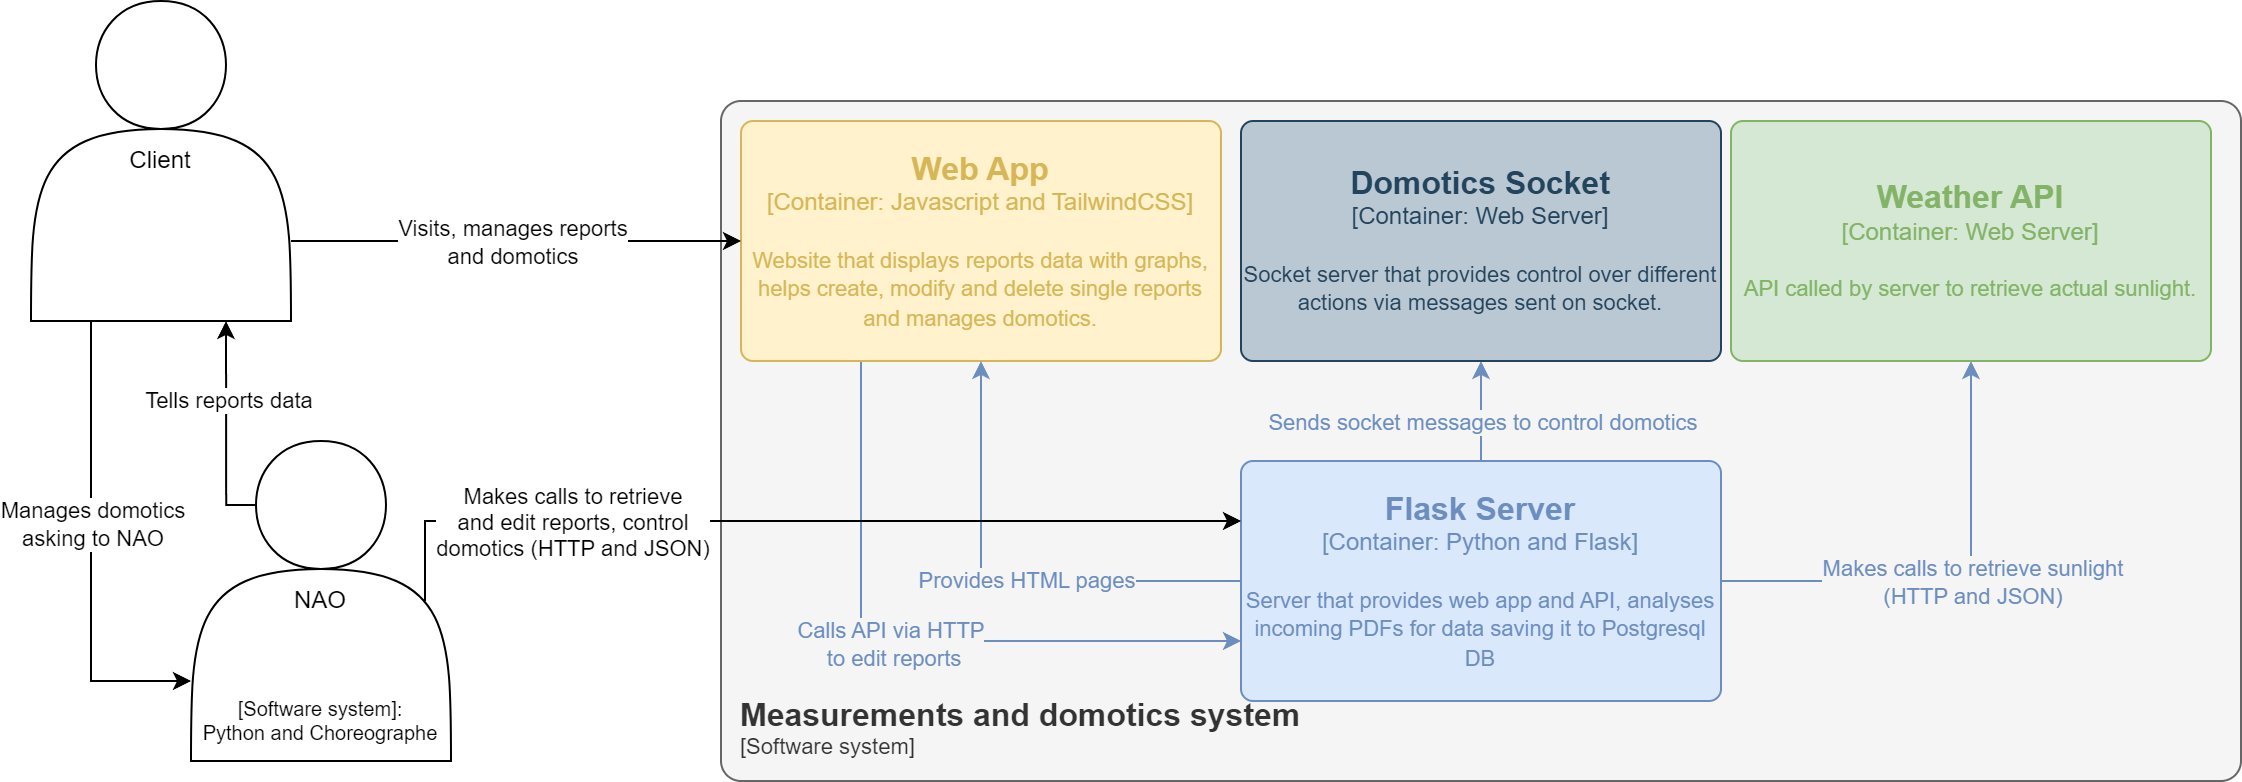
\includegraphics[scale=0.17]{figures/architecture_domotics.png}
    \caption{NAO domotics project architecture}
    \label{fig:my_label}
\end{figure}

\bigskip
\subsection{The sensor}\label{sec:domotics_sensor}
\vspace{5pt}
A significant part of the project was being able to analyse the environment and collect data of the CO2 concentration, temperature and humidity. At first the team wanted to use an Arduino that had to connect to the \hyperref[sec:domotics_server]{HTTP server}. Lots of problems were encountered so we decided to buy an \emph{off-the-shelf} sensor. This guaranteed more precise results with the drawback that they were exported to the PDF.\\ 
\\In order to analyse these data a device that extracted the PDF and sent it to the server was needed. Initially the team wanted to connect the sensor to one of the USB of NAO but without root permission drives couldn't be mounted to the humanoid, making it impossible to access any external memory from NAO. It was therefore decided to use a \hyperref[sec:domotics_app]{mobile app}.\\

\bigskip
\subsection{The App}\label{sec:domotics_app}
\vspace{5pt}
This mobile app is used to load the PDF and send it to the server. It was used because there was no way to connect the \hyperref[sec:domotics_sensor]{sensor} directly to the server. This is a device that helps transfer the sensor's data to the server adding other useful measurements that can't be made with the sensor. This app is written in \emph{Flutter} to make it cross-platform and flexible. It includes a file picker and an input to insert the \emph{number of people} in the room. When sending the file it adds to the request the \emph{light} values measured with the phone sensor. The app also lists all the data stored in the \hyperref[sec:domotics_server]{server}.\\

\begin{figure}[H]
    \centering
    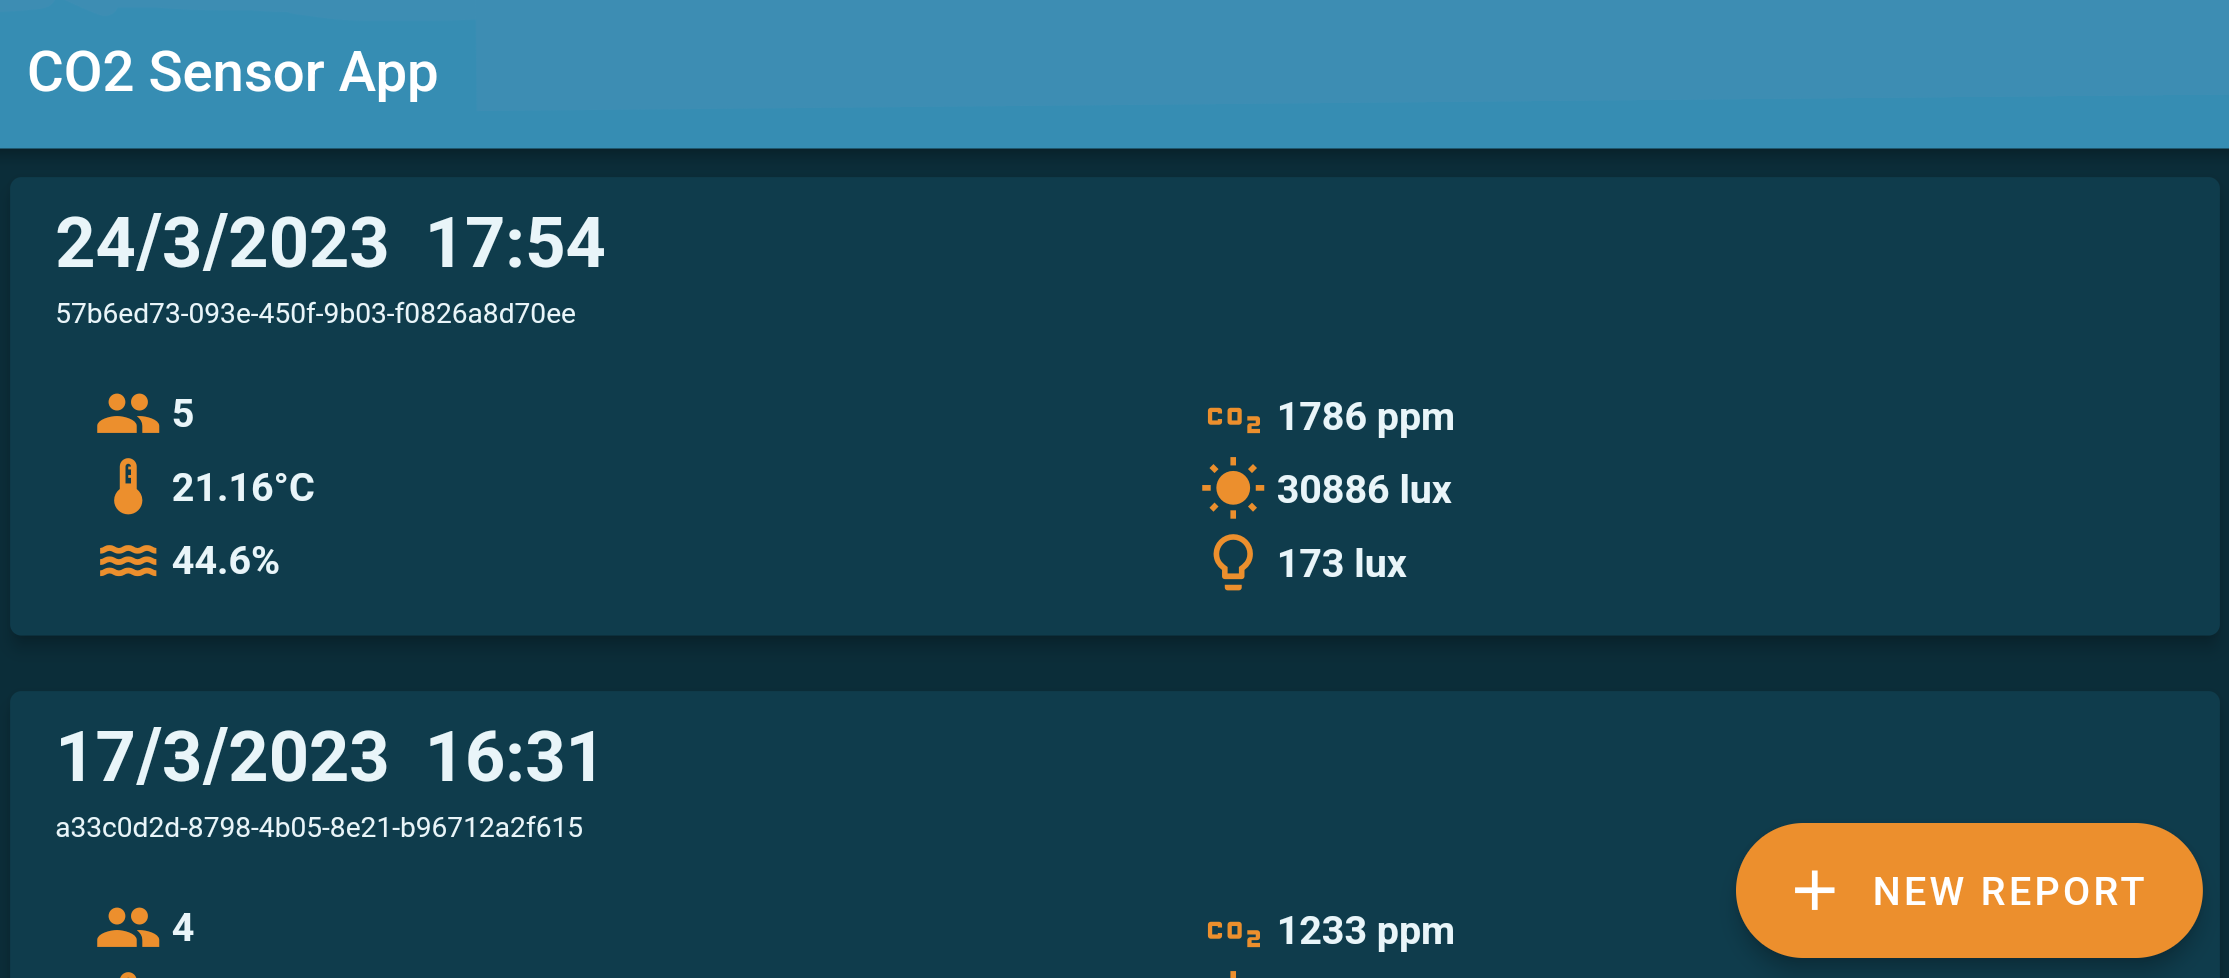
\includegraphics[scale=0.17]{figures/domotics_app.png}
    \caption{Domotics application}
    \label{fig:app_domotica}
\end{figure}


\subsection{NAO}\label{sec:domotics_nao}
NAO is the central point of the project. It is connected to the \hyperref[sec:domotics_server]{HTTP server} and receives the collected environmental data used by NAO to understand which calls to make to the server. With \hyperref[sec:domotics_domotics_server]{control domotics} NAO tells the user what it is doing. NAO has the functionality to be used as a "smart home speaker" like \emph{"Alexa"}: the end user can ask NAO to make adjustments to the domotics controlling it directly. When receiving new data NAO communicates them to the user and based on various \emph{thresholds} it can control the smart devices.

\vspace{12pt}
\subsection{HTTP Server}\label{sec:domotics_server}
The central point where all the data of the project is managed, this is a complex part written in Python that \hyperref[sec:domotics_pdf_analysis]{analyses PDFs}, adds missing information, hosts a \hyperref[sec:domotics_web_app]{Web App} that views and manage data and hosts a \hyperref[sec:domotics_rest_api]{Rest API} to connect all the clients like the \hyperref[sec:domotics_app]{mobile app} and \hyperref[sec:domotics_nao]{NAO}. The initial idea was to run this server on NAO but the latest software versions removed the ability to \emph{root} the robot and install Python packages, it was later decided to run this server on a \emph{Raspberry PI} with a \emph{fixed IP} to make it accessible to every client on the network.

\subsubsection{Web App}\label{sec:domotics_web_app}
An important part of the server is the web app that it hosts: the HTML pages are populated with \href{https://jinja.palletsprojects.com/en/3.1.x/}{Jinja} and are sent using \href{https://flask.palletsprojects.com/en/2.2.x/}{Flask}. This library is responsible of running the \hyperref[sec:domotics_rest_api]{Rest server} that provides data in \emph{JSON} format. In this web app the data of the reports is viewable with a \emph{graph} or as a \emph{list}, every report is \emph{editable} and \emph{deletable} and it is possible to \emph{add new reports}. 

\begin{figure}[H]
    \centering
    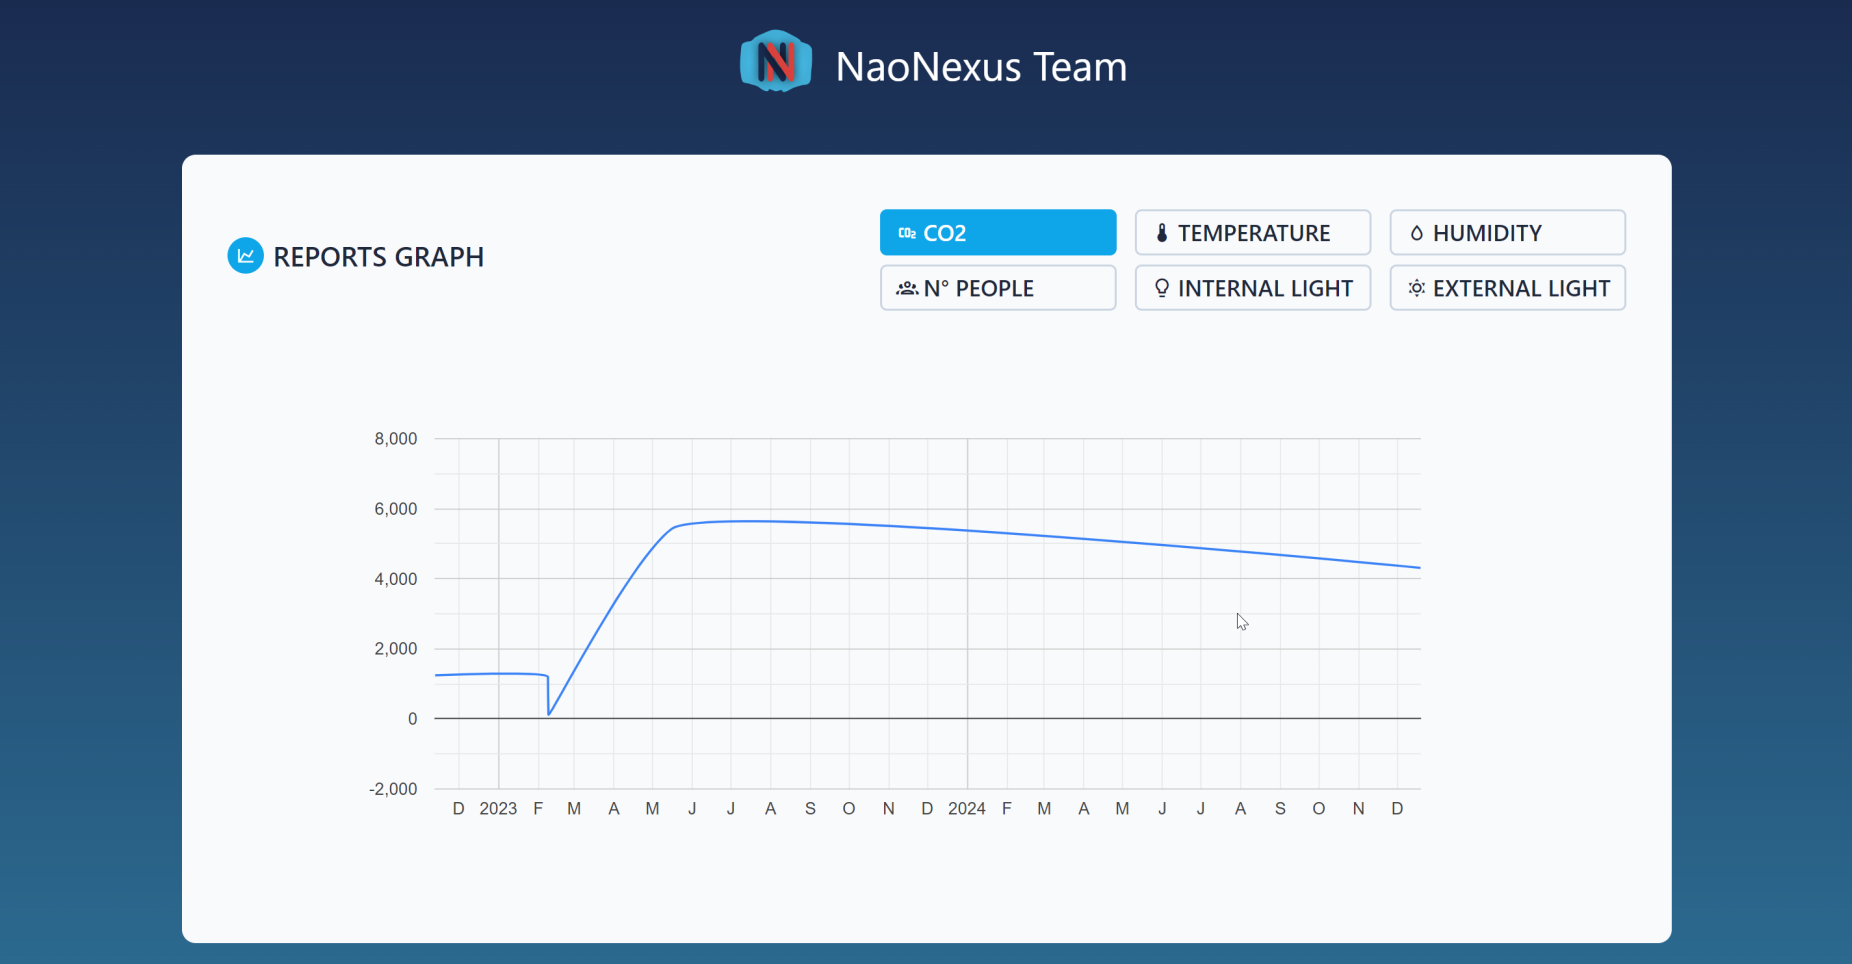
\includegraphics[scale=0.26]{figures/web_app_summary.png}
    \caption{Screen to see reports summary}
    \label{fig:webb_app_summary}
\end{figure}

\vspace{8pt}
\subsubsection{Rest API}\label{sec:domotics_rest_api}
\textit{The documentation for the API can be found \href{https://naonexus.notion.site/Domotics-server-22721767d69a43a6badeafcaf546b3d2}{here}.}\\
\\The Rest API facilitates the exchange of data between all the connected clients, which are then sent via \emph{JSON} using \emph{HTTP} and are accessible through multiple endpoints. This rest server is written in \hyperref{https://flask.palletsprojects.com/en/2.2.x/}{Flask} as the \hyperref[sec:domotics_web_app]{App}.

\begin{figure}[H]
    \centering
    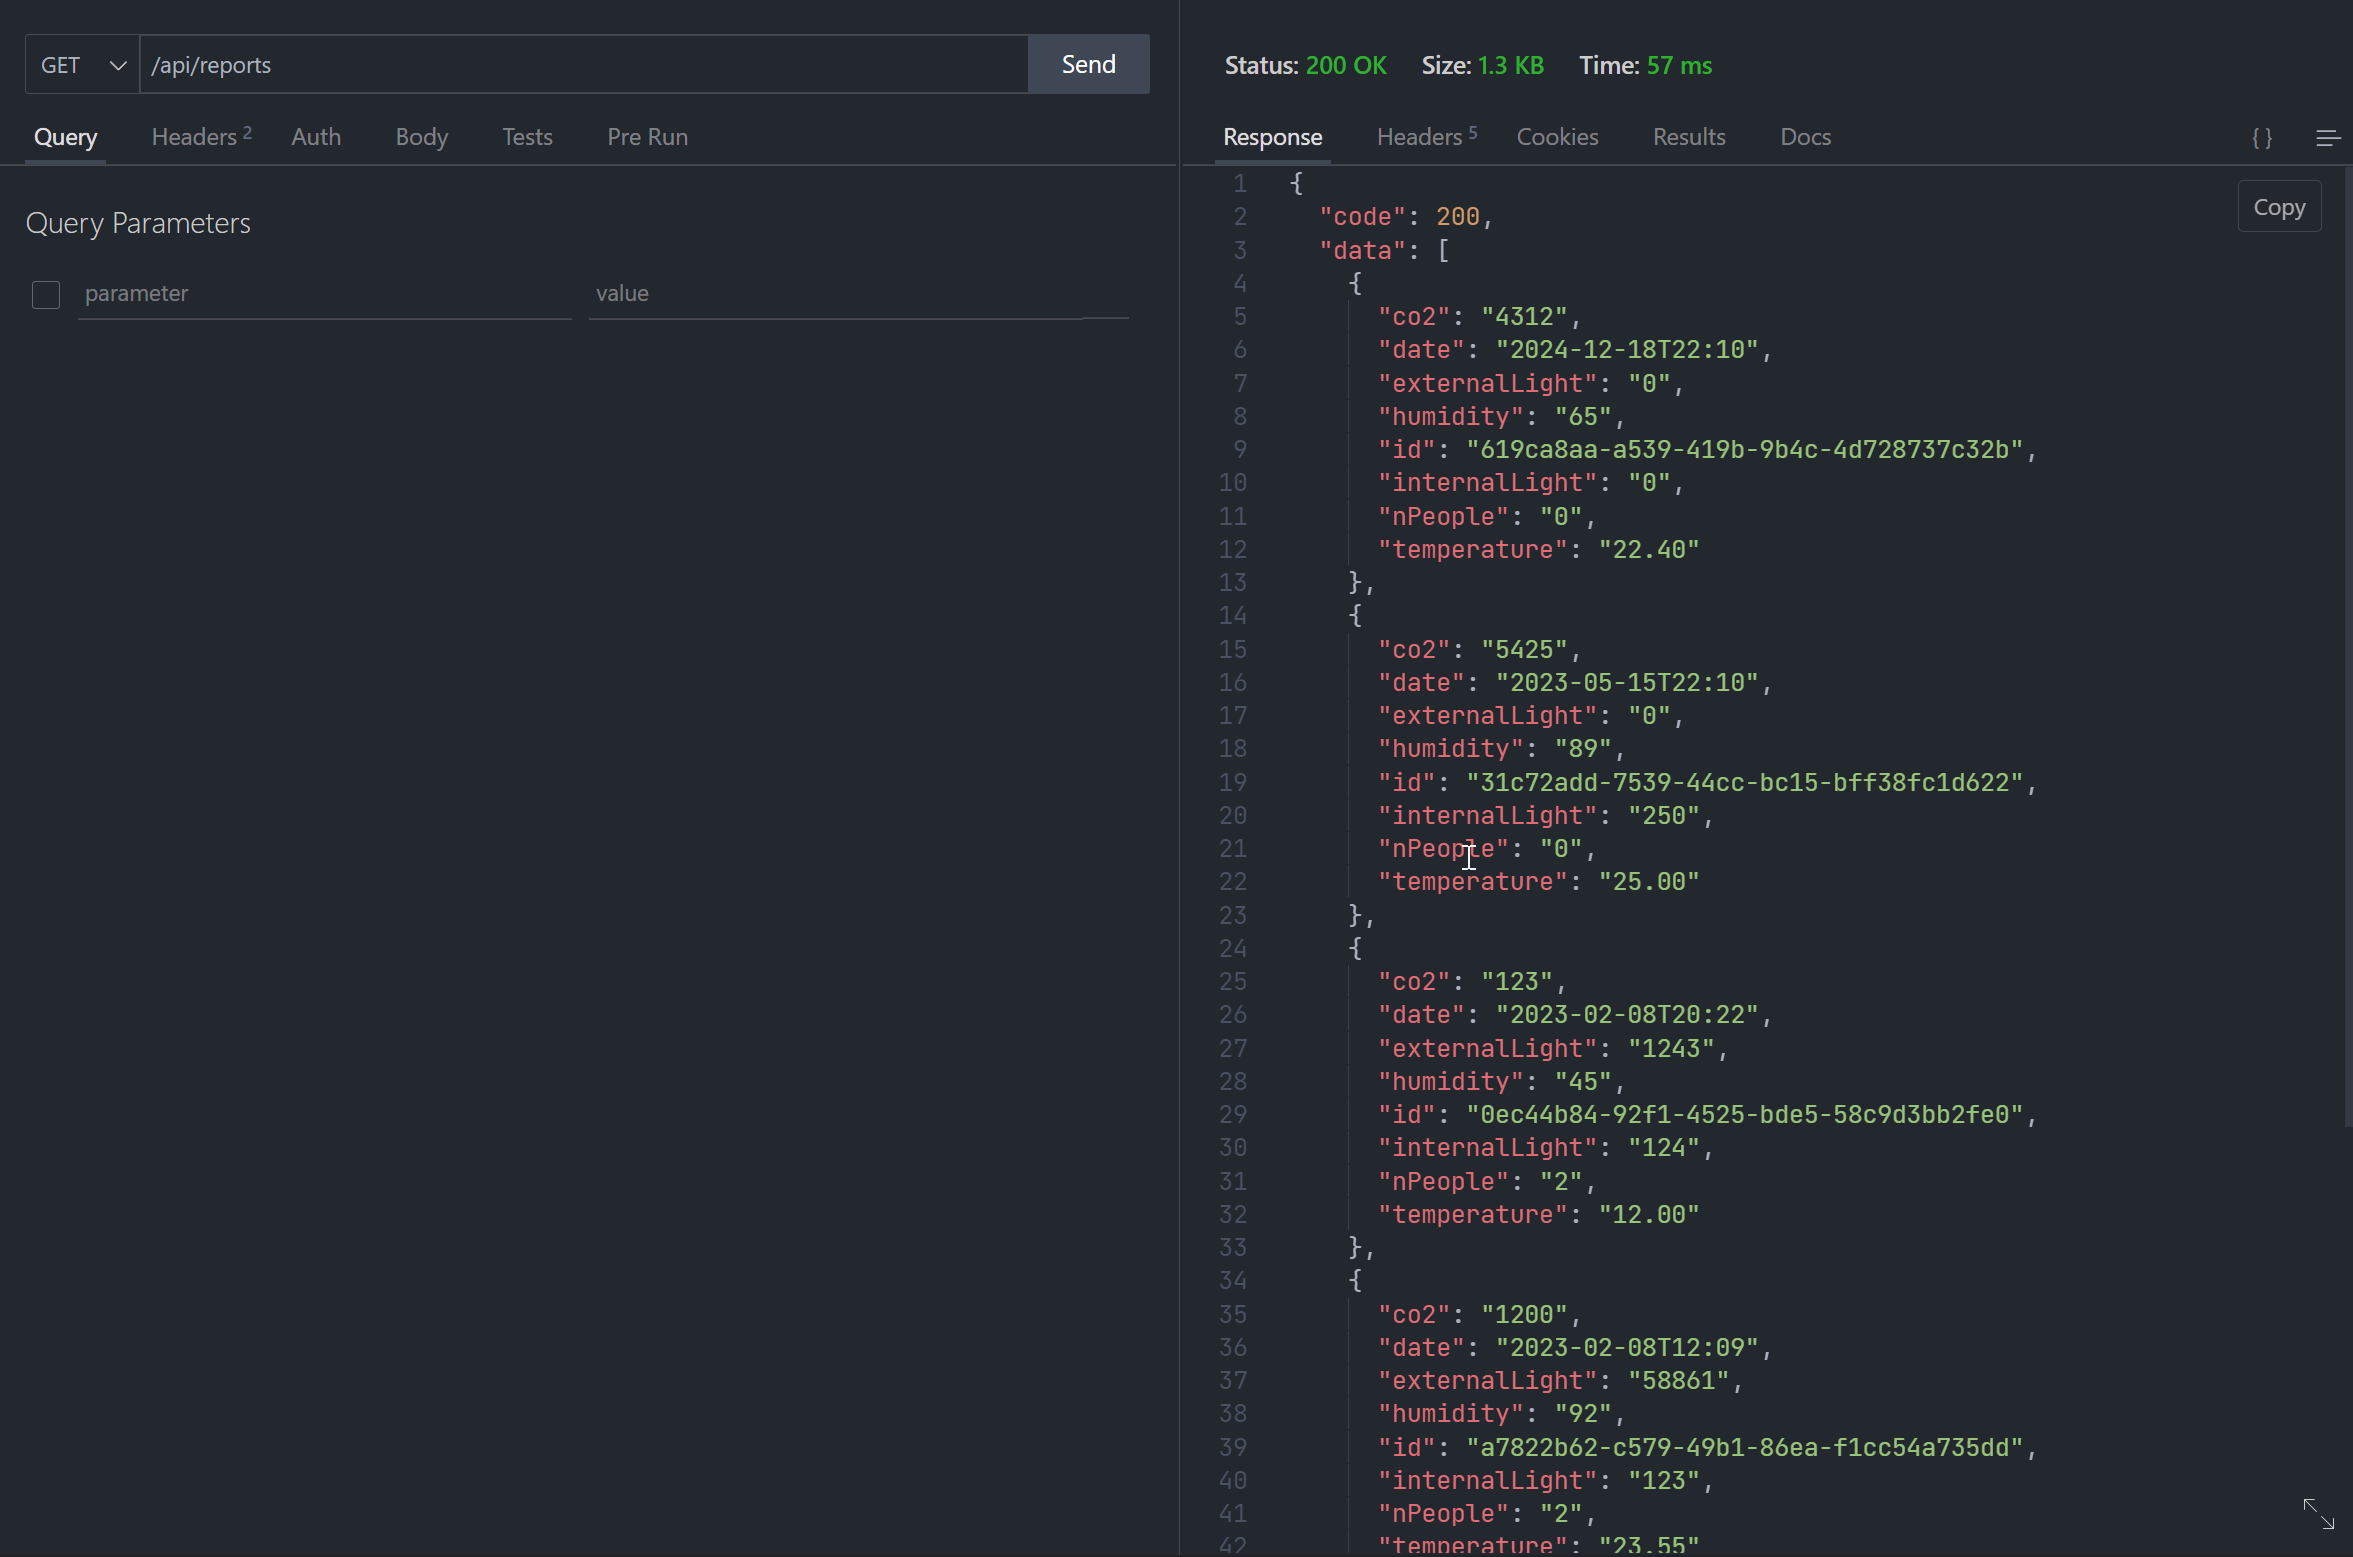
\includegraphics[scale=0.36]{figures/sample_api_response.png}
    \caption{Sample Rest API response}
    \label{fig:rest_api_reponse}
\end{figure}

\vspace{8pt}
\subsubsection{PDF Analysis}\label{sec:domotics_pdf_analysis}
In order to analyse the PDF it was necessary to use the \href{https://pypdf2.readthedocs.io/en/3.0.0/}{pyPDF2} library, which allowed the conversion of the file created by the \hyperref[sec:domotics_sensor]{CO2 sensor} into a string. The parameters were difficult to individuate but after removing \emph{spaces} and \emph{line breaks} the program was able to find useful values by searching for \emph{keywords} allocated in specific points of the PDF. In this way it is possible to extract various data from the PDF like: date of the measurement, CO2, temperature and humidity.

\vspace{8pt}
\subsubsection{Domotics control}\label{sec:domotics_domotics_server}
To control the lights the server was connected via \emph{Telnet} to the domotics server of the building. After some difficulties trying to find the right commands and thanks to \emph{Amperia}'s guidance, it was possible to understand the appropriate unique codes assigned to \emph{lights}, \emph{LIMs}, \emph{blinds} and \emph{thermostats} in a specific environment, in order to control them through the \emph{Telnet} connection. This connection brought the \hyperref[sec:domotics_server]{HTTP Server} to become a \emph{client} for the domotics server in order for it to control the connected devices.

\vspace{8pt}
\subsubsection{External light analysis}
The measurements of the internal light is retrieved from the \hyperref[sec:domotics_sensor]{sensor} but the external sunlight cannot be measured by the app. The first idea was to add an \emph{Arduino} sensor externally, this couldn't be applied to every possible situation and building. The solution was to call an external API (\href{https://open-meteo.com/}{Open meteo}), this API returns solar irradiance in $\frac{W}{m^2}$ that is then converted in $lux$ by the server. 

\bigskip 
\section{NAO AS A GUIDE TO SOLAREDGE}\label{sec:solaredge_project}

This project involves NAO to interact with the clients of the partner \emph{Amperia}, it asks for details of the building and generates a project for a solar transition with the website Solaredge making sustainability accessible to everyone. It includes two phases: an initial phase where \hyperref[sec:solaredge_nao]{NAO} asks questions to the customer and inserts the answers in the website asking the customer to do it when it isn't able to control the website and a second phase where NAO tells all the results achievable from the project and the impact that it has on the Earth. The project contains multiple elements:\\

\begin{itemize}
    \item \hyperref[sec:solaedge_server]{HTTP Server}: a Rest server that communicates with NAO and controls the website inserting requested data
    \item \hyperref[sec:solaredge_nao]{NAO}: a humanoid robot that asks for details and sends the answers to the server that analyses them. It spells out loud the result from the analysed data, generated with Solaredge website.
\end{itemize}

\begin{figure}[!htbp]
    \centering
    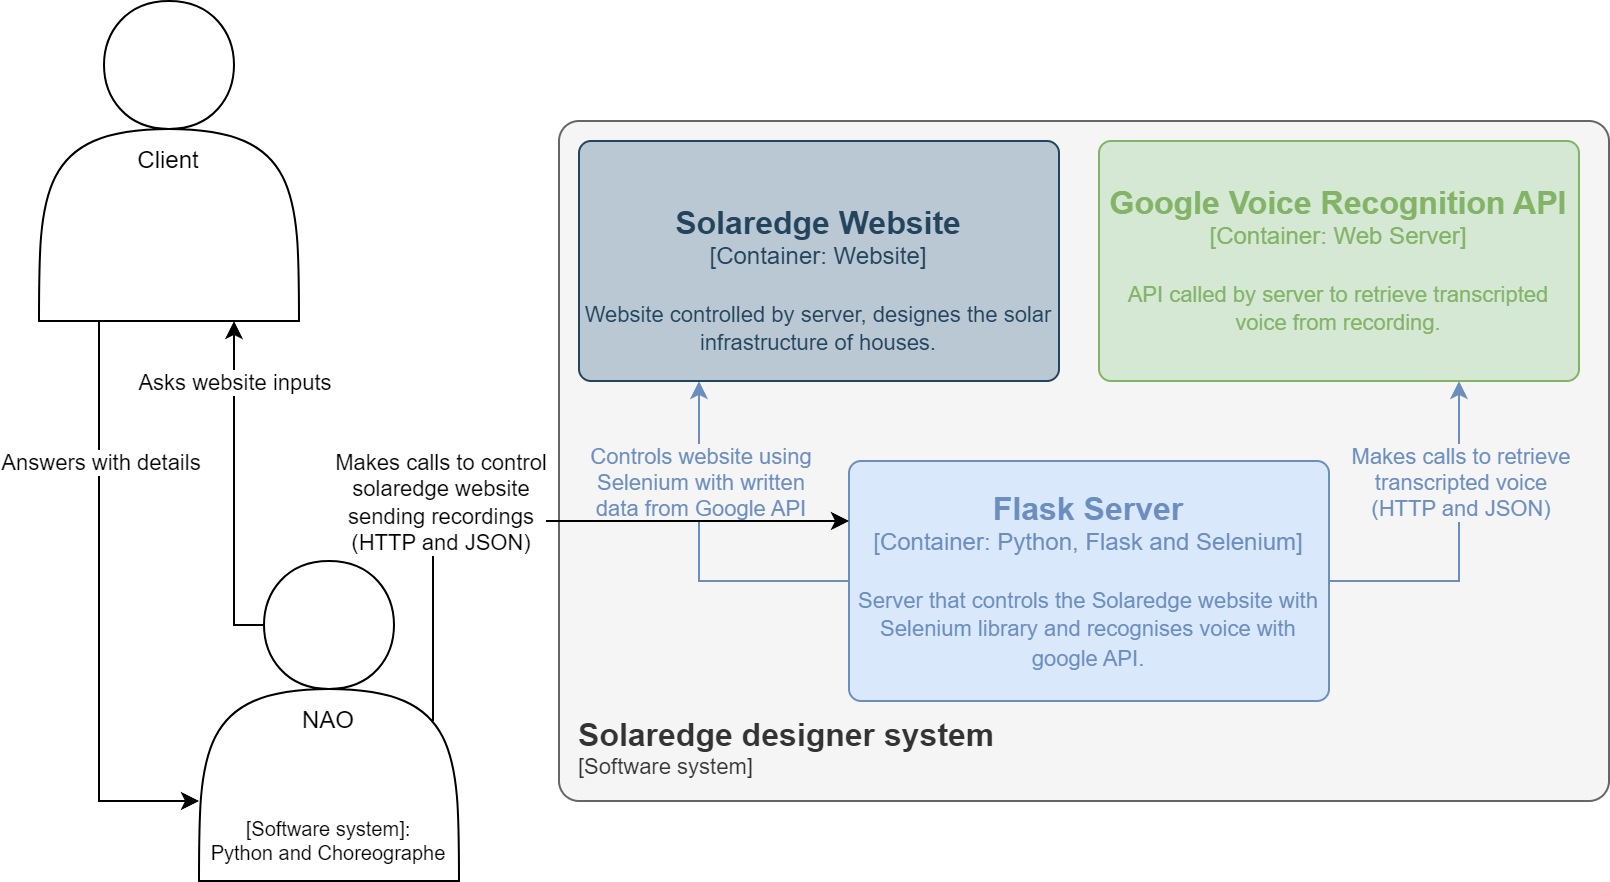
\includegraphics[scale=0.23]{figures/architecture_solaredge.png}
    \caption{Solaredge architecture}
    \label{fig:architecture_solaredge}
\end{figure}

\subsection{NAO}\label{sec:solaredge_nao}
NAO is an essential part of this project, it handles the interaction with the customer that wants to configure its solar panel installation. The initial idea was to add the libraries to control Solaredge website directly as a \emph{package} of NAO's Python but the same problem of the \\\hyperref[sec:domotics_server]{other project} was encountered: there wasn't a way to install packages. The solution was to add a computer as a \emph{server} and access the website on it making the website accessible to the user. When extracting the customer answers a problem was encountered: NAO voice recognition works only on known words but the inputs from the user could have been anything. It was then decided to register the response from NAO and send the WAV file to the server to analyse it. NAO makes questions and registers the answers of the customer and then procceds to send them as WAV to the \hyperref[sec:solaedge_server]{server}. When the project is completed the robot says aloud the results expected from the project.

\vspace{12pt}
\subsection{HTTP Server}\label{sec:solaedge_server}
The central point where all the data of the project are stored, this is a complex part written in Python that communicates with NAO receiving voice registration. It then \hyperref[sec:solaredge_voice_recognition]{analyse these registrations} by extracting the transcription that are \hyperref[sec:solaredge_website_control]{inserted in Solaredge website}. It includes various static and dynamic endpoints to manage data and is written using \href{https://flask.palletsprojects.com/en/2.2.x/}{Flask}. Similarly to the other project the \hyperref[sec:solaedge_server]{server} isn't run directly on NAO but on an external PC, this makes the code flexible and helps the user to adjust the inserted data and access the website.

\vspace{8pt}
\subsubsection{Rest API}\label{sec:solaredge_rest_api}
\textit{The documentation for the API can be found \href{https://naonexus.notion.site/Solaredge-server-1bae2ae87b4d407b82f5a50bbfe3d87c}{here}.}\\
\\This Rest API manages the traffic of data from NAO to the server and the other way round. It includes various endpoints and uses HTTP protocol, furthermore WAV files registered by NAO are parsed and inserted in Solaredge website.

\vspace{8pt}
\subsubsection{Voice Recognition}\label{sec:solaredge_voice_recognition}
The transcription of the voice is done using Python's library \href{https://pypi.org/project/SpeechRecognition/}{SpeechRecognition}, it uses \emph{Google}'s models and returns a text from an audio file. It is used to transform NAO's registrations into text to be entered in the website. The audio file given to this library presents two channels that include the \emph{right} and \emph{left} microphones of NAO.

\vspace{8pt}
\subsubsection{Solaredge website Control}\label{sec:solaredge_website_control}
\href{https://www.selenium.dev/documentation/}{Selenium} is a Python library containing numerous instructions that allow for a direct interaction with a local browser of choice. This tool can scour through the HTML code of a website and, in doing so, finding, selecting and interacting with specific graphic elements within the code itself (such as textboxes, lists, links etc.). It \emph{automatizes} both the \emph{extraction} and \emph{importation} of the data, optimizing the process and making it more efficient. This library is fundamental in inserting the parsed questions extracted from the dialogue between \hyperref[sec:solaredge_nao]{NAO} and the customer.

\section{Team and Authors}\label{sec:team_authors}
The NaoNexus team is divided in two sections: \emph{coding} and \emph{social}. The components who worked on the social part of the project made sure to represent the NaoNexus experience at its best, creating and posting new content everyday in order to highlight the major progresses made by the group during these months. The social sub-team had a key role in presenting the project with videos, pictures, reels and \href{https://www.tiktok.com/@naonexus}{TikToks} to post on our socials and the Naonexus \href{https://www.naonexus.altervista.org}{website}.

\bigskip
\noindent
The coding division took care of the robotics project per se, developing the code and working with the technologies and methodologies previously explained.\\

\subsection{CODING DIVISION}

\noindent\emph{Riccardo Antonelli - Team Leader}\\
\emph{Francesco Bernardi}\\
\emph{Elisa D'Iseppi}\\
\emph{Filippo Buso}\\
\emph{Edoardo Polfranceschi}\\

\bigskip

\subsection{SOCIAL DIVISION}

\noindent\emph{Alberto Rubini - Team Leader}\\
\emph{Davide Masini}\\
\emph{Antonio Galati}\\
\emph{Arianna Antonelli}\\


\begin{figure}[b]
    \centering
    
\includegraphics[scale=0.04]{figures/logo.png}
    \label{fig:logo_con_scritta1}
\end{figure}


%\vspace{70pt}
%\listoffigures
\end{document}